\documentclass[a4paper,12pt]{scrartcl}
\usepackage[utf8]{inputenc}
\usepackage[french]{babel}
\usepackage[T1]{fontenc}
\usepackage{amsmath}
\usepackage{color}
\usepackage{graphicx}
\usepackage{isotope}
\usepackage{units}
\usepackage{float}
\usepackage{scrpage2}
  

\title{TP Cesire \isotope[13]{C} en RMN}
\author{Mona Dentler, Sabine Engelhardt et Laura Hilpert}
%mitautor Michel Bardet, Sabine Herdiger
\publishers{Université Joseph Fourier, CEA Grenoble}

 \begin{document}

 \pagestyle{empty}
 \begin{center}
  \makeatletter
   %\titlefont
  \@subject
  \vspace{2cm}

  \Huge
  TP Cesire \isotope[13]{C} en RMN\newline
  \vspace{1cm}
  \Large


  \@author
  \newline
  \@publishers


  \@date
  \makeatother
 \end{center}
 \vfill

 \begin{abstract}
  Le but de ce TP Cesire est de comprendre comment faire un RMN des solides. On sait déjà très bien faire un RMN de solution, mais pour un solide il y a quelques problèmes. Un solide est inhomogène et il y a la force dipôlaire qui dérange la mesure car les atomes sont fortement couplés. En solution cette force se moyenne à zéro.\\ 
  Comment alors obtenir un bon image d'un solide? D'abord nous avons appris un peu de la théorie d'un RMN et sutout les solutions pour faire un RMN d'un solide pour ensuite les vérifier en mesurant. 
 \end{abstract}
 \newpage
\pagestyle{scrheadings}
 \tableofcontents

 \section{RMN}
  \subsection{RMN d'une solution}

  \subsection{Problématique d'un RMN d'un solide}
   
  \subsection{Solutions}
   \subsubsection{Découplage}

   \subsubsection{Übertragung Magnetisierung}

   \subsubsection{Rotation de l'angle magique}

   \subsubsection{Puissance de Hartmann-Hahn}
 
 

 \section{Dispositif expérimental}
  \subsection{Montage expérimental}
   Nous avons usé deux différent dispositif experimental, leur seule différence est que celui pour la mesure de la cellulose donne la possibilité des mesures plus précises.

   Le dispositif se constiste d'un électroaimant pour le champ magnétique exterieur dans lequel se trouve l'échantillon. L'échantillon est mis dans un petit roteur avec peu d'air pour ne pas déranger la mesure. Ce roteur est placé dans la bobine qui se trouve à l'interieur refroidi du électroaimant. Cette bobine est \textcolor{red}{Sender} et sondes des ondes radio en même temps. 

   On peut choisir la fréquence de la rotation et le reste de la mesure est dirigé par l'ordinateur. Les dates sont directement transferé à l'ordinateur pour donner la possibilté d'y faire une transformation Fourier des dates pour obtenir le spectre.

   Le deuxième dispositif donne la possibilité de mesurer plus précise à cause de deux choses:
   \begin{itemize}
    \item L'interieur est plus froid, donc il y a moins de dérangement
    \item La rotation est plus vite, alors la structure est plus homogène
   \end{itemize}


  \subsection{Préliminaire} 
   Pour voir que l'échatillon est bien placé et le dispositif est bien calibré il faut d'abord faire un \flqq wob\frqq. \c Ca veut dire qu'on regarde l'énergie absorbé en fonction de la fréquence. On connaît la fréquence des atomes de l'échantillon qui on veut mesurer, ici nous avons usé la fréquence pour le \isotope[13]{C} et la fréquence pour le H. Cette fréquence est envoyé sur l'échantillon est on obeserve que le système absorbe l'énergie sauf à la fréquence ou on veut mesurer. 

   Si on ne fait pas cela avant la mesure on peut avoir deux choses qu'on ne veut pas. Premièrement on ne voit rien pendant la mesure car la réponse, donc la fréquence de la réponse, est absorbé et deuxièment ce qu'on veut surtout pas il y a la possibilité que l'énergie pas absorbée détruit la sonde, parce qu'elle est trop grande.

   \subsection{Influence des paramètres sur la mesure}
    \subsubsection{Nombre de scans}
     La différence signal/ bruit est proporionnel à $\sqrt{ns}$, donc pour améliorer le résultat par deux il faut avoir un nombre de scans $nd$ 4 fois plus grand.

    \subsubsection{Fréquence de la rotation}

    \subsubsection{Temps de contact}

    \subsubsection{Puissance des signaux}

 \section{Glycerine}
  Nous avons fait ces expériment pour verifier les différents théorie pour obtenir un beau spectre.

  \subsection{Rotation de l'angle magique}
   La première expérience était de changé la fréquence de la rotation de l'angle magique. On a dit que le solide semble plus homogène le plus vite il est tourné. Nous avons fait une mesure avec une rotation à \unit[4]{kHz}, puis \unit[3]{kHz}, \unit[2]{kHz}, \unit[1]{kHz}, \unit[0,75]{kHz}, \unit[0,5]{kHz},\unit[0,2]{kHz} et sans rotation. Dès la mesure de \unit[0,75]{kHz} nous avons augmenté le nombre de scans de 4 à 16 pour obtenir un meilleur spectre. 
   \begin{figure}[H]
    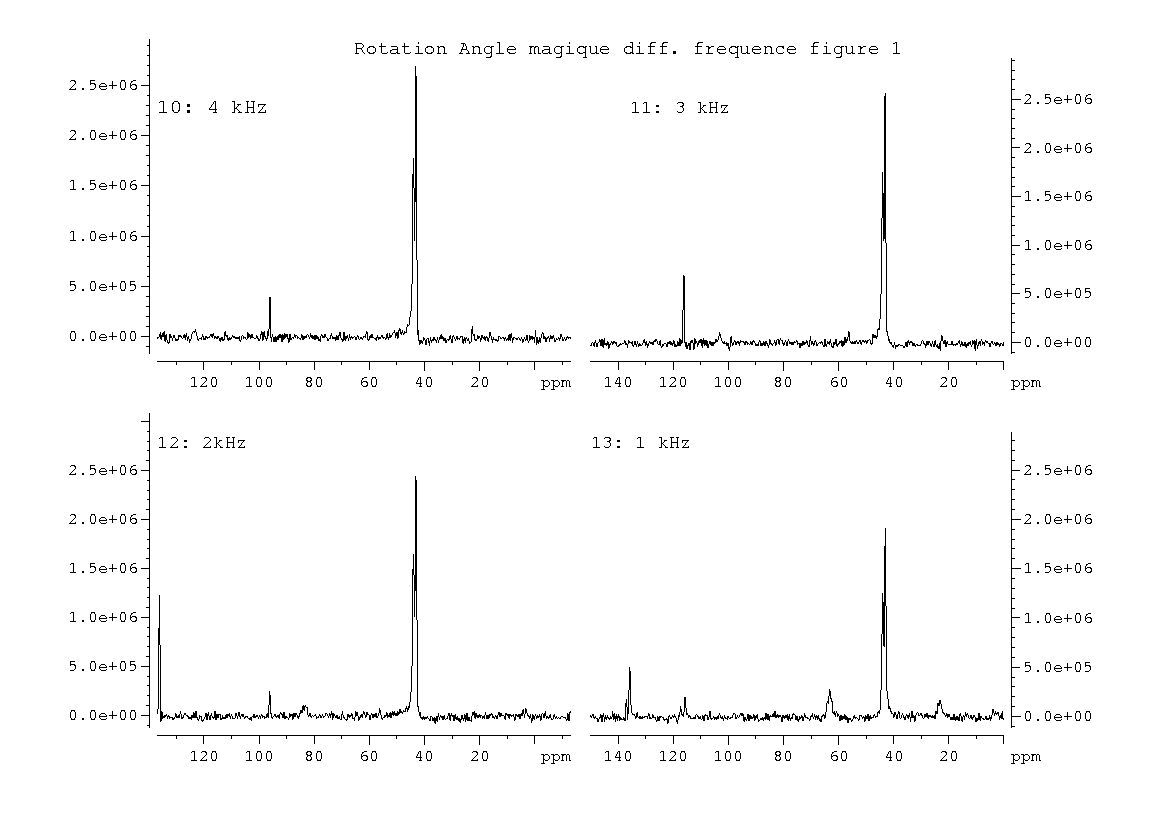
\includegraphics[width=\textwidth]{bilder/rotation.png}
    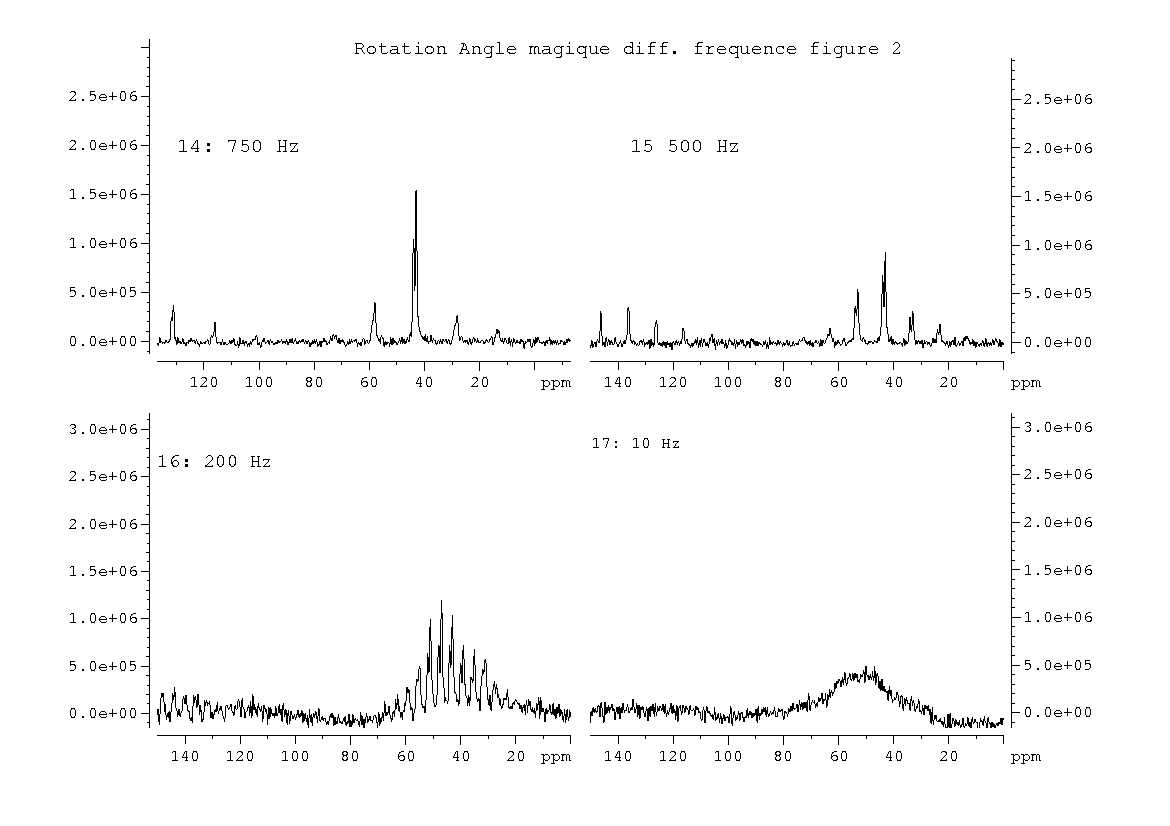
\includegraphics[width=\textwidth]{bilder/rotation2.png}
    \caption{\label{rotation}Les spectres pour les différents fréquences.}
   \end{figure}
   \paragraph{Interprétation}
    On voit bien dans les spectres de la figure \ref{rotation} à la p. \pageref{rotation} que les signaux qu'on veut obtenir se dimunue porportionnelement à la fréquence de la rotation. C'est à cause de la nombre de pics qui augmente. La même \textcolor{red}{Anzahl} de signaux est detéctés, mais il sont distribue sur différents pics. Dans le premier spectre avec \unit[4]{kHz} on ne voit que les deux pics fines assez grands de \textcolor{red}{welche?} C et C. Dans le deuxième spectre on voit déjá plusieurs autres pics, les bandes rotationelles. On sait que ce sont des bandes rotationnelles car la \textcolor{red}{Abstand} entre le signal vraie et ses bandes rotationelles est $d=n\cdot f_{rot}$ avec $f_{rot}$ la fréquence de la rotation de l'angle magique. Dans le dernier spectre on ne voit rien. Il n' y a qu'un pic très large avec le maximum même pas à la position correcte. Le deuxième pic, le plus petit, n'est plus vue.

   \paragraph{Conclusion}
    Donc nous avons vu que c'est vraie quand diminue les artefacts causé par l'inhomogenité \textcolor{red}{???} du solide avec la rotation de l'angle magique. 

  \subsection{Temps de contact}
   Le temps de contact c'est le temps pendant laquelle on transfere \textcolor{red}{die Quermagnetisierung} des atomes d'H aux atomes de C.

  \subsection{Puissance de Hartmann-Hahn}
 
 

 \section{Graines de salade}
  \subsection{Condition liquide}
 
  \subsection{CP masse}

  \subsection{DEPT ?}
   Spektrum mit gekippten Peaks, wenn an ungerader Anzahl von Protonen, irgenwie mit Kopplung

  \subsection{2D-Spektrum}
   wie Dept, aber Entkopplung glaube ich später
 
 

 \section{Cellulose}
  \subsection{Spectre \isotope[13]{C}}
   nicht erkennbar was was ist, am Ende Spektum nochmal zeigen +beschriftet  

  \subsection{Spectre H}
   Wasser peak und Artefakt, bandes rotationelles

  \subsection{Spin-diffusion}
  
  \subsection{Inadequate}

  \subsection{Hetcore}
 
   abgeschnitten Spinning sidebands, noch da fehler wegen zu kurz gemessen = Signal abgeschnitten
 
 

 \section{Conclusion}
 
 


\end{document}
